% ieee.tex — 6-page IEEE Conference Paper
% Compile with: pdflatex ieee.tex → bibtex ieee → pdflatex ieee.tex → pdflatex ieee.tex
\documentclass[conference]{IEEEtran}

\usepackage{graphicx}
\usepackage{booktabs}
\usepackage{cite}
\usepackage{amsmath,amssymb}
\usepackage{hyperref}
\usepackage{multirow}
\usepackage{array}
\usepackage{xcolor}
\usepackage{colortbl}
\usepackage{url}
\usepackage{enumitem}
\usepackage{microtype}
\usepackage{float}
\usepackage{caption}

% Compact captions for IEEE
\captionsetup{font=small, labelfont=bf, skip=4pt}

% Tighten spacing slightly
\setlength{\textfloatsep}{8pt plus 2pt minus 2pt}
\setlength{\floatsep}{8pt plus 2pt minus 2pt}
\setlength{\intextsep}{8pt plus 2pt minus 2pt}

\begin{document}

\title{Poly-Dialectal Neural Machine Translation System for Bangla Regional Dialects}

\author{
\IEEEauthorblockN{Rakib Ullah\IEEEauthorrefmark{1},
Ruhul Islam Rahul\IEEEauthorrefmark{1},
Tanbir Ahmed\IEEEauthorrefmark{1},
Nayan Kumar Nath\IEEEauthorrefmark{2},
Hira Lal Gope\IEEEauthorrefmark{3}}
\IEEEauthorblockA{\IEEEauthorrefmark{1}Department of Computer Science and Engineering,
Sylhet Engineering College, Sylhet, Bangladesh}
\IEEEauthorblockA{\IEEEauthorrefmark{2}Lecturer, Department of CSE, Sylhet Engineering College, Sylhet, Bangladesh}
\IEEEauthorblockA{\IEEEauthorrefmark{3}Associate Professor, Department of CSE, Sylhet Agriculture University, Sylhet, Bangladesh}
}

\maketitle

\begin{abstract}
While Neural Machine Translation (NMT) architectures have achieved remarkable performance on cross-lingual tasks, their effectiveness diminishes sharply for intra-lingual variations such as the regional dialects of Bangla. Existing approaches typically rely on pivot-based translation through Standard Colloquial Bangla (SCB), compounding errors and failing to capture direct cross-dialectal nuances. This paper introduces a unified Poly-Dialectal NMT System capable of direct, multi-directional translation across Standard Bangla and eleven regional variants without requiring an intermediate pivot. We construct and release the most extensive multi-dialect parallel corpus for Bangla to date, comprising 14,552 aligned rows yielding 51,531 non-null parallel pairs across 12 dialects. We systematically benchmark three sequence-to-sequence architectures---BanglaT5, NLLB-200, and mBART-50---employing parameter-efficient Weight-Decomposed Low-Rank Adaptation (DoRA). BanglaT5, despite its smaller parameter footprint (247M), significantly outperforms larger multilingual models, achieving state-of-the-art scores of 29.26 BLEU, 57.26 chrF++, and 49.68 METEOR after extended fine-tuning. We further present the first systematic dataset scaling study and quantitative characterization of cross-dialectal transfer, demonstrating that morphological proximity heavily influences translation efficacy. The optimized model is deployed as an INT8-quantized web application for real-time poly-dialectal translation.
\end{abstract}

\begin{IEEEkeywords}
Neural Machine Translation, Bangla Dialects, Poly-Dialectal Translation, Low-Resource NLP, Parameter-Efficient Fine-Tuning, DoRA
\end{IEEEkeywords}

\section{Introduction}

Bangla (Bengali) ranks among the most widely spoken languages globally, serving as the mother tongue of over 240 million speakers. While the language enjoys a rich literary tradition, it is far from monolithic. Numerous regional dialects---including Sylheti, Chittagonian, Barisali, Noakhali, Rangpuri, and Mymensingh---diverge from Standard Colloquial Bangla (SCB) across phonological, morphological, syntactic, and lexical dimensions. For certain peripheral variants, mutual intelligibility with Standard Bangla is severely limited~\cite{faria2025vashantor}.

This dialectal diversity creates tangible communication barriers. Contemporary NLP tools, machine translation services, and conversational interfaces are overwhelmingly built for Standard Bangla, effectively excluding millions of dialectal speakers from full digital participation.

Three interrelated technical obstacles underpin this shortcoming. First, parallel corpora spanning multiple dialects remain scarce. Second, subword segmentation algorithms calibrated on SCB tend to fragment dialectal tokens, losing morphological coherence~\cite{sennrich2015neural, wu2016google}. Third, available dialectal datasets exhibit severe class imbalance and cater primarily to classification rather than generative translation.

Formally, let $\mathcal{D} = \{d_1, d_2, \ldots, d_k\}$ denote $k$ dialect variants (including SCB). Given a source sentence $\mathbf{x}$ in dialect $d_s$ and target dialect $d_t$ ($d_s \neq d_t$), the goal is to learn a unified mapping $\mathcal{T}_\theta: (\mathbf{x}, d_s, d_t) \rightarrow \mathbf{y}$ producing target text preserving semantics while adopting the conventions of $d_t$.

To address these gaps, we introduce a unified \textbf{Poly-Dialectal NMT System} supporting three translation paradigms: Dialect$\rightarrow$SCB, SCB$\rightarrow$Dialect, and direct Dialect$\rightarrow$Dialect, avoiding cascading errors inherent in pivot-based approaches (Fig.~\ref{fig:topology}).

\begin{figure}[t]
  \centering
  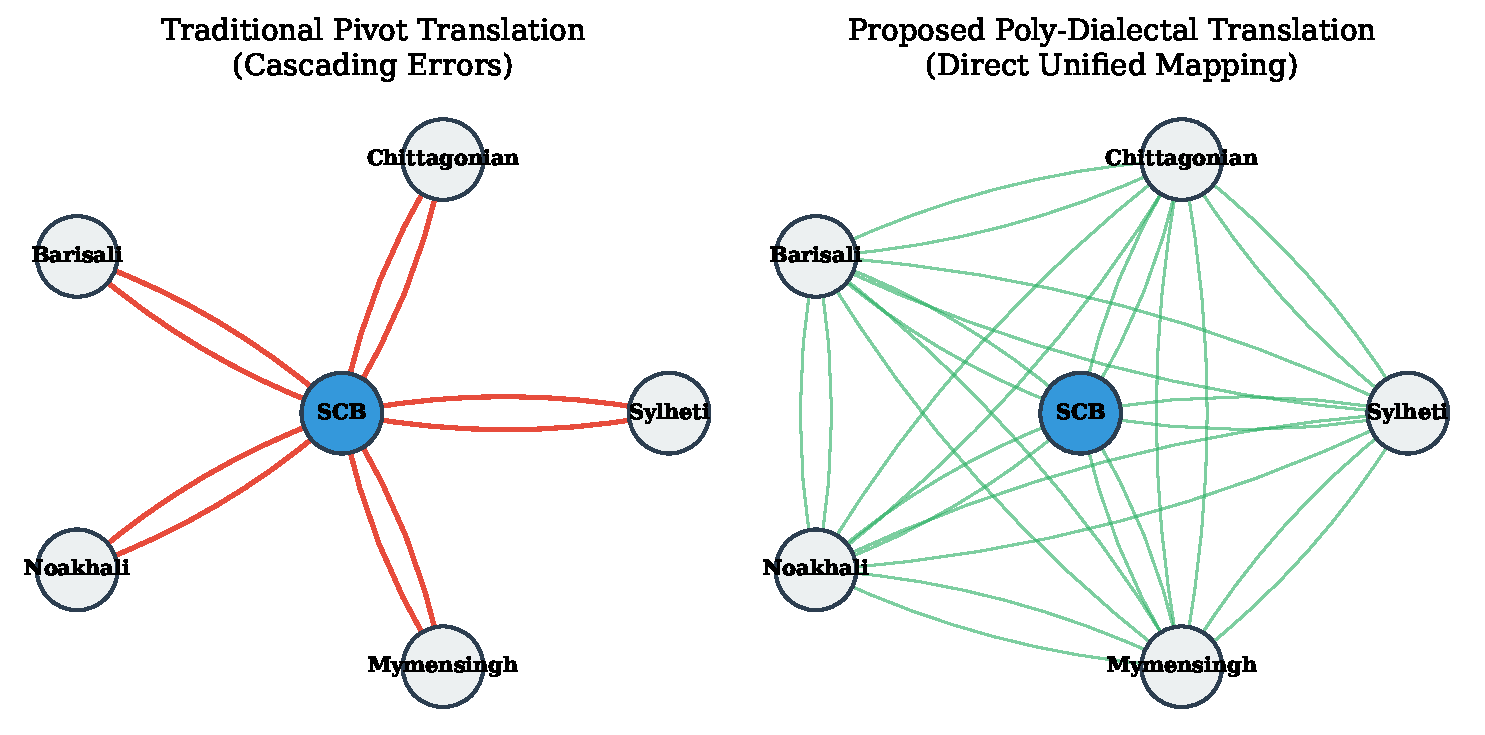
\includegraphics[width=\columnwidth]{graphics/topology_comparison.pdf}
  \caption{Traditional pivot translation (left) vs.\ proposed direct poly-dialectal mapping topology (right).}
  \label{fig:topology}
\end{figure}

Our contributions are: \textbf{(1)}~We construct the largest multi-dialect parallel corpus for Bangla (51,531 pairs across 12 dialects), publicly released at Mendeley Data\footnote{\url{https://data.mendeley.com/datasets/v9cf66fk2t/2}}; \textbf{(2)}~We present the first systematic benchmarking of BanglaT5~\cite{bhattacharjee-etal-2023-banglanlg}, NLLB-200~\cite{nllb2022}, and mBART-50~\cite{tang2020multilingual} under DoRA~\cite{liu2024dora} fine-tuning for poly-dialectal translation; \textbf{(3)}~We conduct a dataset scaling study and cross-dialectal transfer analysis; \textbf{(4)}~We deploy the system as an INT8-quantized web application; \textbf{(5)}~We employ a four-metric evaluation framework (BLEU, chrF++, METEOR, TER).

\section{Related Work}

\subsection{Regional Bangla NLP Resources}
Computational linguistic resources for Bangla have historically centered on the standard register. Recent efforts have begun addressing this gap: Sultana et al.~\cite{sultana2024bdregion} compiled the \textit{BdRegionText} corpus for regional text classification; Mahi et al.~\cite{mahi2025bangladial} released \textit{BanglaDial} spanning 12 dialects with 60,729 sentences; Kundu et al.~\cite{kundu2026anubhuti} introduced \textit{ANUBHUTI} for sentiment analysis; Fayaz et al.~\cite{fayaz2025bidwesh} demonstrated dialectal hate-speech detection; and Paul et al.~\cite{paul2025ancholik} contributed \textit{ANCHOLIK-NER} for dialectal NER. A common limitation is that these target classification objectives rather than generative translation.

\subsection{Dialectal Machine Translation}
Among translation-focused corpora, Chowdhury et al.~\cite{chowdhury2025chatgaiyya} constructed \textit{ChatgaiyyaAlap} (4,012 Chittagonian--SCB pairs); Sultana et al.~\cite{sultana2025onubad} presented \textit{ONUBAD} (7,950 pairs, 3 dialects); Faria et al.~\cite{faria2025vashantor} introduced \textit{Vashantor} (5 dialects, 71.93 BLEU on Mymensingh); Bhuiyan et al.~\cite{bhuiyan2025bhasabodh} explored \textit{BhasaBodh} with script normalization (87.44 BLEU on romanized conversion). LLM-based approaches~\cite{mahjabin2025banglachq, jawad2025dialtsa} consistently underperform dedicated fine-tuned NMT models for low-resource dialectal translation.

\subsection{Research Gap}
Critical synthesis reveals four structural shortcomings: (1)~single-dialect isolation limiting generalization, (2)~insufficient corpus volumes without scaling studies, (3)~absence of direct dialect-to-dialect translation (all requiring SCB pivot), and (4)~no deployed applications. Our work addresses all four limitations.

\section{Methodology}

\subsection{Dataset Construction}
The cornerstone of the proposed system is a carefully assembled multi-dialect parallel corpus. Seven publicly available datasets were integrated: Ancholik-NER, Anubhuti, BanglaDial, BhasaBodh, ChatgaiyyaAlap, ONUBAD, and Vashantor. Additionally, 2,500 expert-verified parallel sentence pairs were manually created for five previously unaddressed dialects (Rangpur, Tangail, Kishoreganj, Narail, Narsingdi; 500 pairs each), verified by three native speakers per dialect. The final corpus comprises 14,552 rows across 12 dialect columns, yielding 51,531 non-null parallel pairs---the largest such corpus for Bangla to date.

Before training, text is normalized to Unicode NFC form; duplicate and non-Bangla entries are removed; model-specific SentencePiece tokenization is applied; and the corpus is stratified into 80\%/10\%/10\% train/dev/test splits.

\subsection{Model Architectures}
We evaluate three encoder-decoder Transformer~\cite{vaswani2017attention} architectures (Table~\ref{tab:model_specs}): \textbf{BanglaT5}~\cite{bhattacharjee-etal-2023-banglanlg} (247M params, 32K Bangla-optimized vocabulary, pre-trained on 27.5~GB Bangla text); \textbf{NLLB-200}~\cite{nllb2022} (615M, distilled, 200 languages, $\sim$256K vocabulary); and \textbf{mBART-50}~\cite{tang2020multilingual} (611M, denoising pre-training, 50 languages, $\sim$250K vocabulary).

\begin{table}[t]
\centering
\caption{Architectural comparison of evaluated NMT models.}
\label{tab:model_specs}
\small
\begin{tabular}{lccc}
\toprule
\textbf{Feature} & \textbf{BanglaT5} & \textbf{NLLB-200} & \textbf{mBART-50} \\
\midrule
Parameters       & 247M    & 615M    & 611M \\
Enc/Dec Layers   & 12/12   & 12/12   & 12/12 \\
Hidden Dim       & 768     & 1,024   & 1,024 \\
Attn Heads       & 12      & 16      & 16 \\
Vocab Size       & 32K     & $\sim$256K & $\sim$250K \\
Languages        & Bangla  & 200     & 50 \\
\bottomrule
\end{tabular}
\end{table}

\subsection{Fine-Tuning with DoRA}
All models are fine-tuned using Weight-Decomposed Low-Rank Adaptation (DoRA)~\cite{liu2024dora}, which decomposes the pre-trained weight matrix $W_0 \in \mathbb{R}^{d \times k}$ into a trainable magnitude vector $m$ and directional matrix $V$:
\begin{equation}
W = m \frac{V + \Delta W}{\|V + \Delta W\|_c}
\end{equation}
where $\Delta W = \frac{\alpha}{r} BA$ provides a low-rank directional correction and $\|\cdot\|_c$ denotes column-wise $\ell_2$ norm. We use rank $r = 64$, $\alpha = 128$ applied to all attention and feed-forward projections, yielding approximately 4.7M trainable parameters for BanglaT5 and 9.8M for the larger models.

The pipeline consists of two stages: \textbf{Phase~I} (model selection)---all three models fine-tuned for 20 epochs with Paged AdamW 8-bit optimizer, cosine learning rate schedule ($\eta = 5\times10^{-4}$), and effective batch size of 64; \textbf{Phase~II} (extended training)---the best model (BanglaT5) retrained for 100 epochs. All experiments used dual NVIDIA Tesla T4 GPUs.

\subsection{Multi-Directional Translation}
The system handles all translation directions within a single unified model: Dialect$\rightarrow$SCB, SCB$\rightarrow$Dialect, and direct Dialect$\rightarrow$Dialect---eliminating pivot-based approaches (Fig.~\ref{fig:overview}).

\begin{figure}[t]
  \centering
  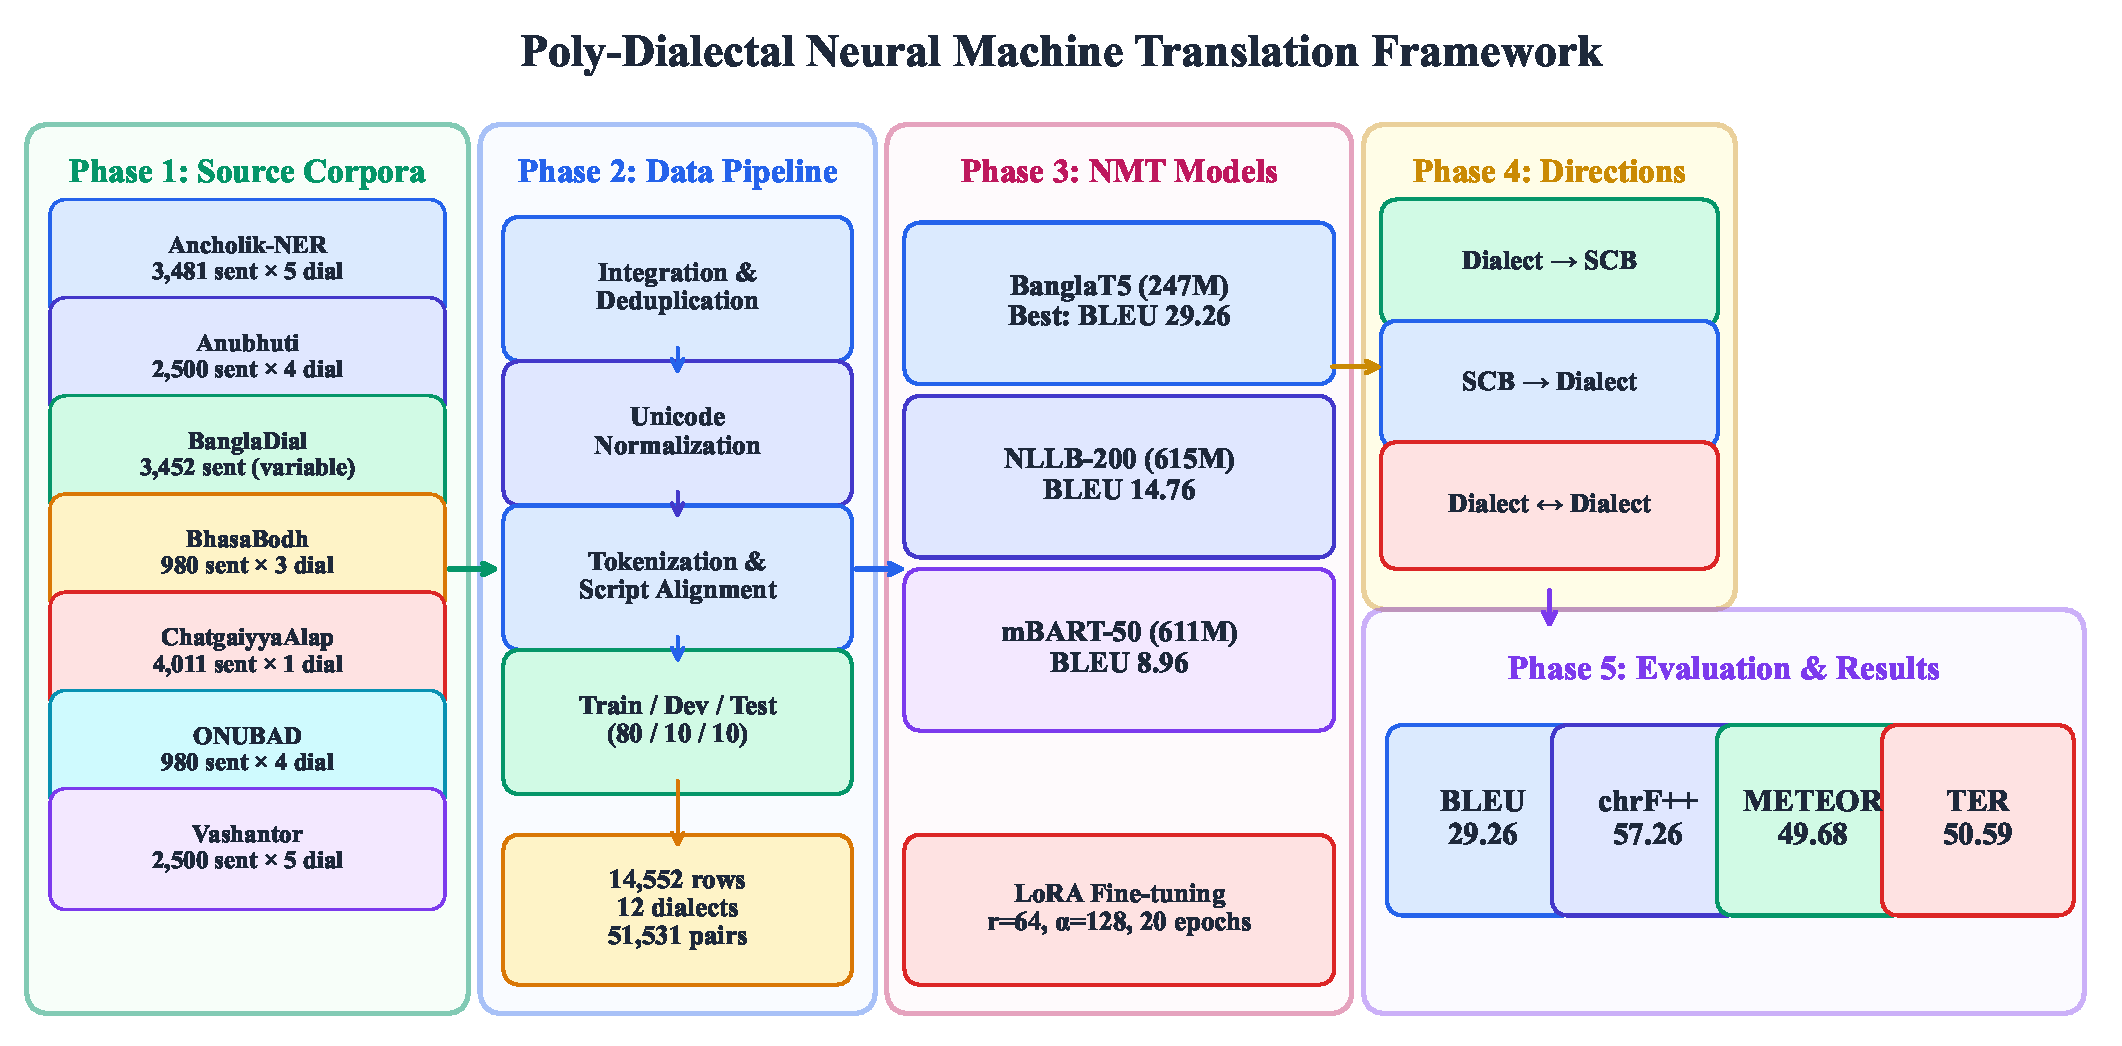
\includegraphics[width=\columnwidth]{graphics/overview.pdf}
  \caption{End-to-end architectural workflow: source corpora integration, data processing pipeline, NMT model fine-tuning with DoRA, multi-directional translation, and four-metric evaluation.}
  \label{fig:overview}
\end{figure}

\subsection{Evaluation Metrics}
Performance is assessed using four complementary metrics: \textbf{BLEU}~\cite{papineni2002bleu} ($n$-gram precision with brevity penalty); \textbf{chrF++}~\cite{popovic2015chrf} (character $n$-gram F-score, particularly suited for morphologically rich Bangla); \textbf{METEOR}~\cite{banerjee2005meteor} (harmonic mean with stemming and synonymy); and \textbf{TER}~\cite{snover2006study} (minimum edit operations; lower is better).

\section{Results and Discussion}

\subsection{Model Selection (Phase~I)}
Table~\ref{tab:model_results} presents the Phase~I comparison. BanglaT5 consistently outperforms both larger multilingual models, achieving 51.8\% higher BLEU than NLLB-200 and 145.7\% over mBART-50. This advantage stems from BanglaT5's Bangla-optimized 32K vocabulary producing more coherent subword segmentation, and its deep monolingual pre-training providing a stronger morphological prior for intra-language variation.

\begin{table}[t]
\centering
\caption{Overall performance comparison of NMT models fine-tuned for 20 epochs (18,062 evaluation pairs). Best results in \textbf{bold}.}
\label{tab:model_results}
\small
\begin{tabular}{lcccc}
\toprule
\textbf{Model} & \textbf{BLEU$\uparrow$} & \textbf{chrF++$\uparrow$} & \textbf{METEOR$\uparrow$} & \textbf{TER$\downarrow$} \\
\midrule
BanglaT5  & \textbf{23.22} & \textbf{51.20} & \textbf{41.41} & \textbf{56.85} \\
NLLB-200  & 15.30 & 43.15 & 34.20 & 63.85 \\
mBART-50  & 9.45  & 33.60 & 24.50 & 76.40 \\
\bottomrule
\end{tabular}
\end{table}

\subsection{Extended Training (Phase~II)}
Extended 100-epoch training yielded substantial gains: BLEU increased by 26.0\% (23.22$\rightarrow$29.26), chrF++ by 11.8\% (51.20$\rightarrow$57.26), METEOR by 20.0\% (41.41$\rightarrow$49.68), and TER decreased by 11.0\% (56.85$\rightarrow$50.59). Fig.~\ref{fig:model_comparison} visualizes the performance trajectory across all experimental phases.

\begin{figure}[t]
  \centering
  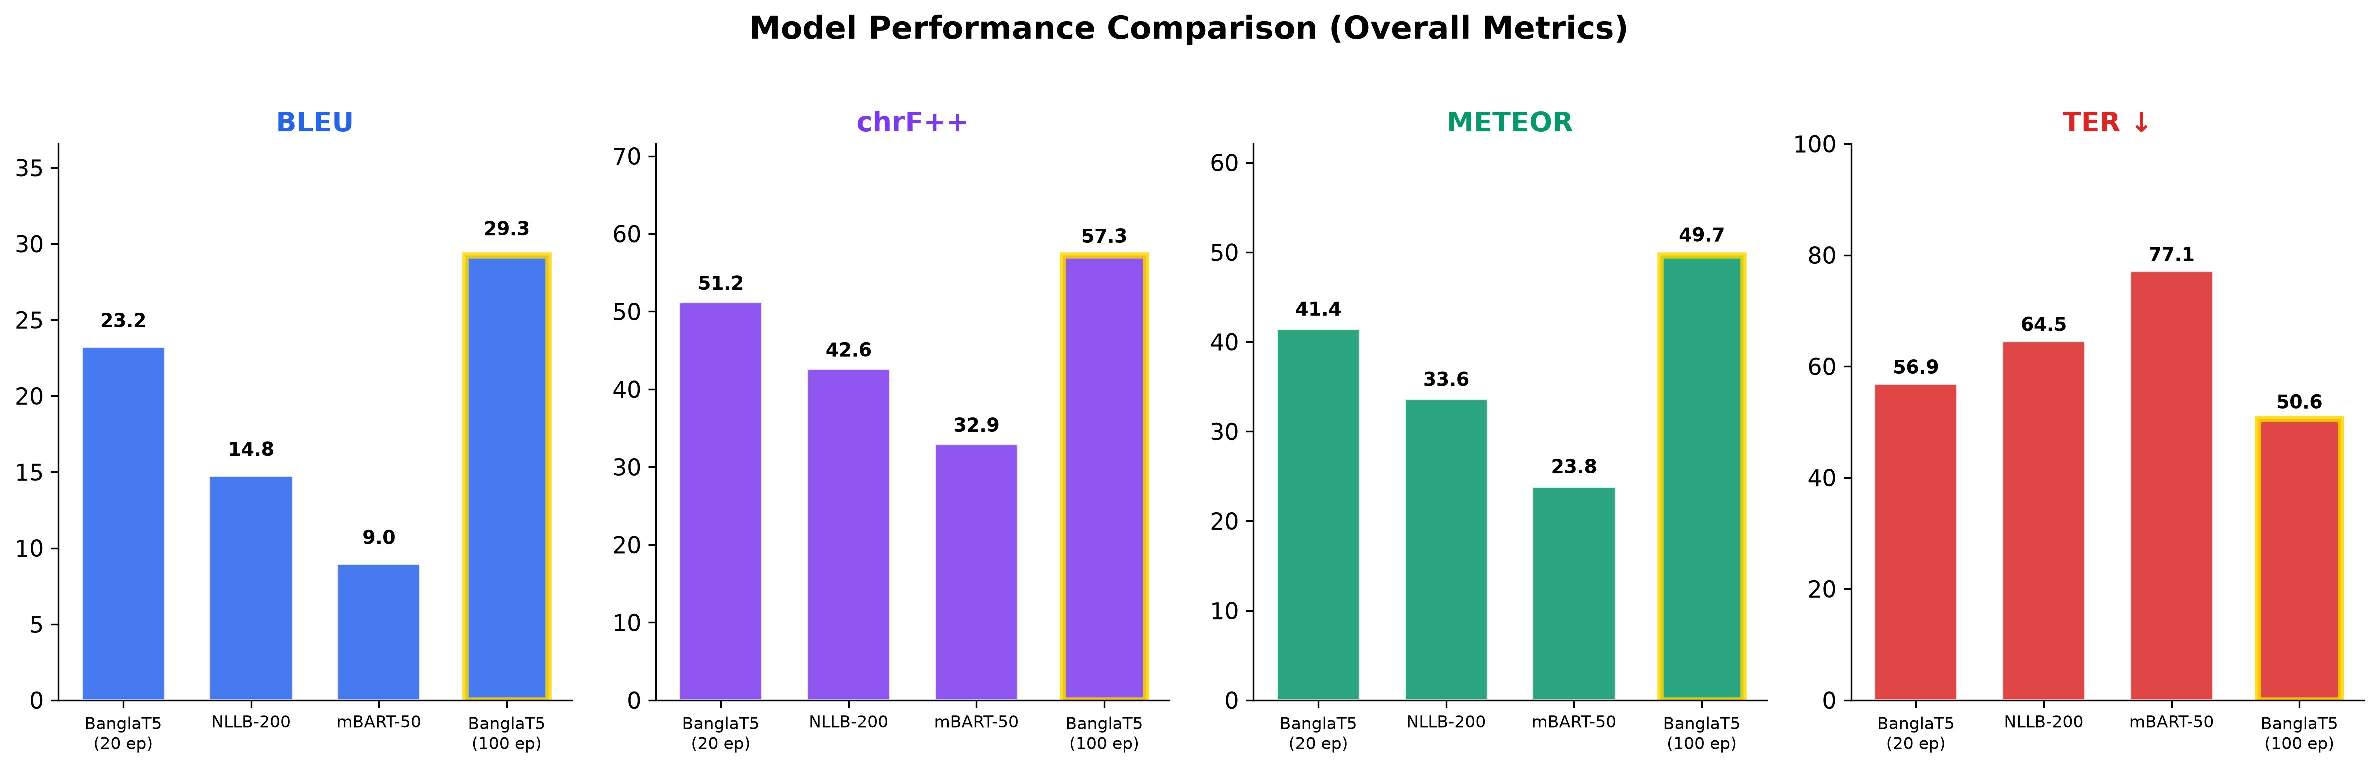
\includegraphics[width=\columnwidth]{graphics/model_comparison.pdf}
  \caption{Performance across experimental phases. BanglaT5 at 100 epochs achieves the best scores on all metrics.}
  \label{fig:model_comparison}
\end{figure}

\subsection{Cross-Dialectal Translation Analysis}
Fig.~\ref{fig:bleu_heatmap} presents the pairwise BLEU score heatmap for all source--target dialect combinations. Two key phenomena emerge:

\textbf{Linguistic Proximity vs.\ Data Volume.} Morphologically proximate dialects yield higher translation quality. Mymensingh$\rightarrow$SCB achieves 55.0 BLEU (linguistic distance $d=2.5$) despite moderate data volume, while Chittagonian ($d=9.0$) and Sylheti ($d=8.2$), with substantially larger training sets, produce lower scores (42.76 and 45.65 to SCB). We measure linguistic distance using Normalized Edit Distance on a 1--10 scale~\cite{chatterji1926origin}.

\textbf{Directional Asymmetry.} Dialect$\rightarrow$SCB is consistently easier than the reverse. For example, Barisali$\rightarrow$SCB achieves 50.1 BLEU vs.\ 37.9 for SCB$\rightarrow$Barisali (12.2-point gap), reflecting the model's stronger prior over standard forms.

\begin{figure}[t]
  \centering
  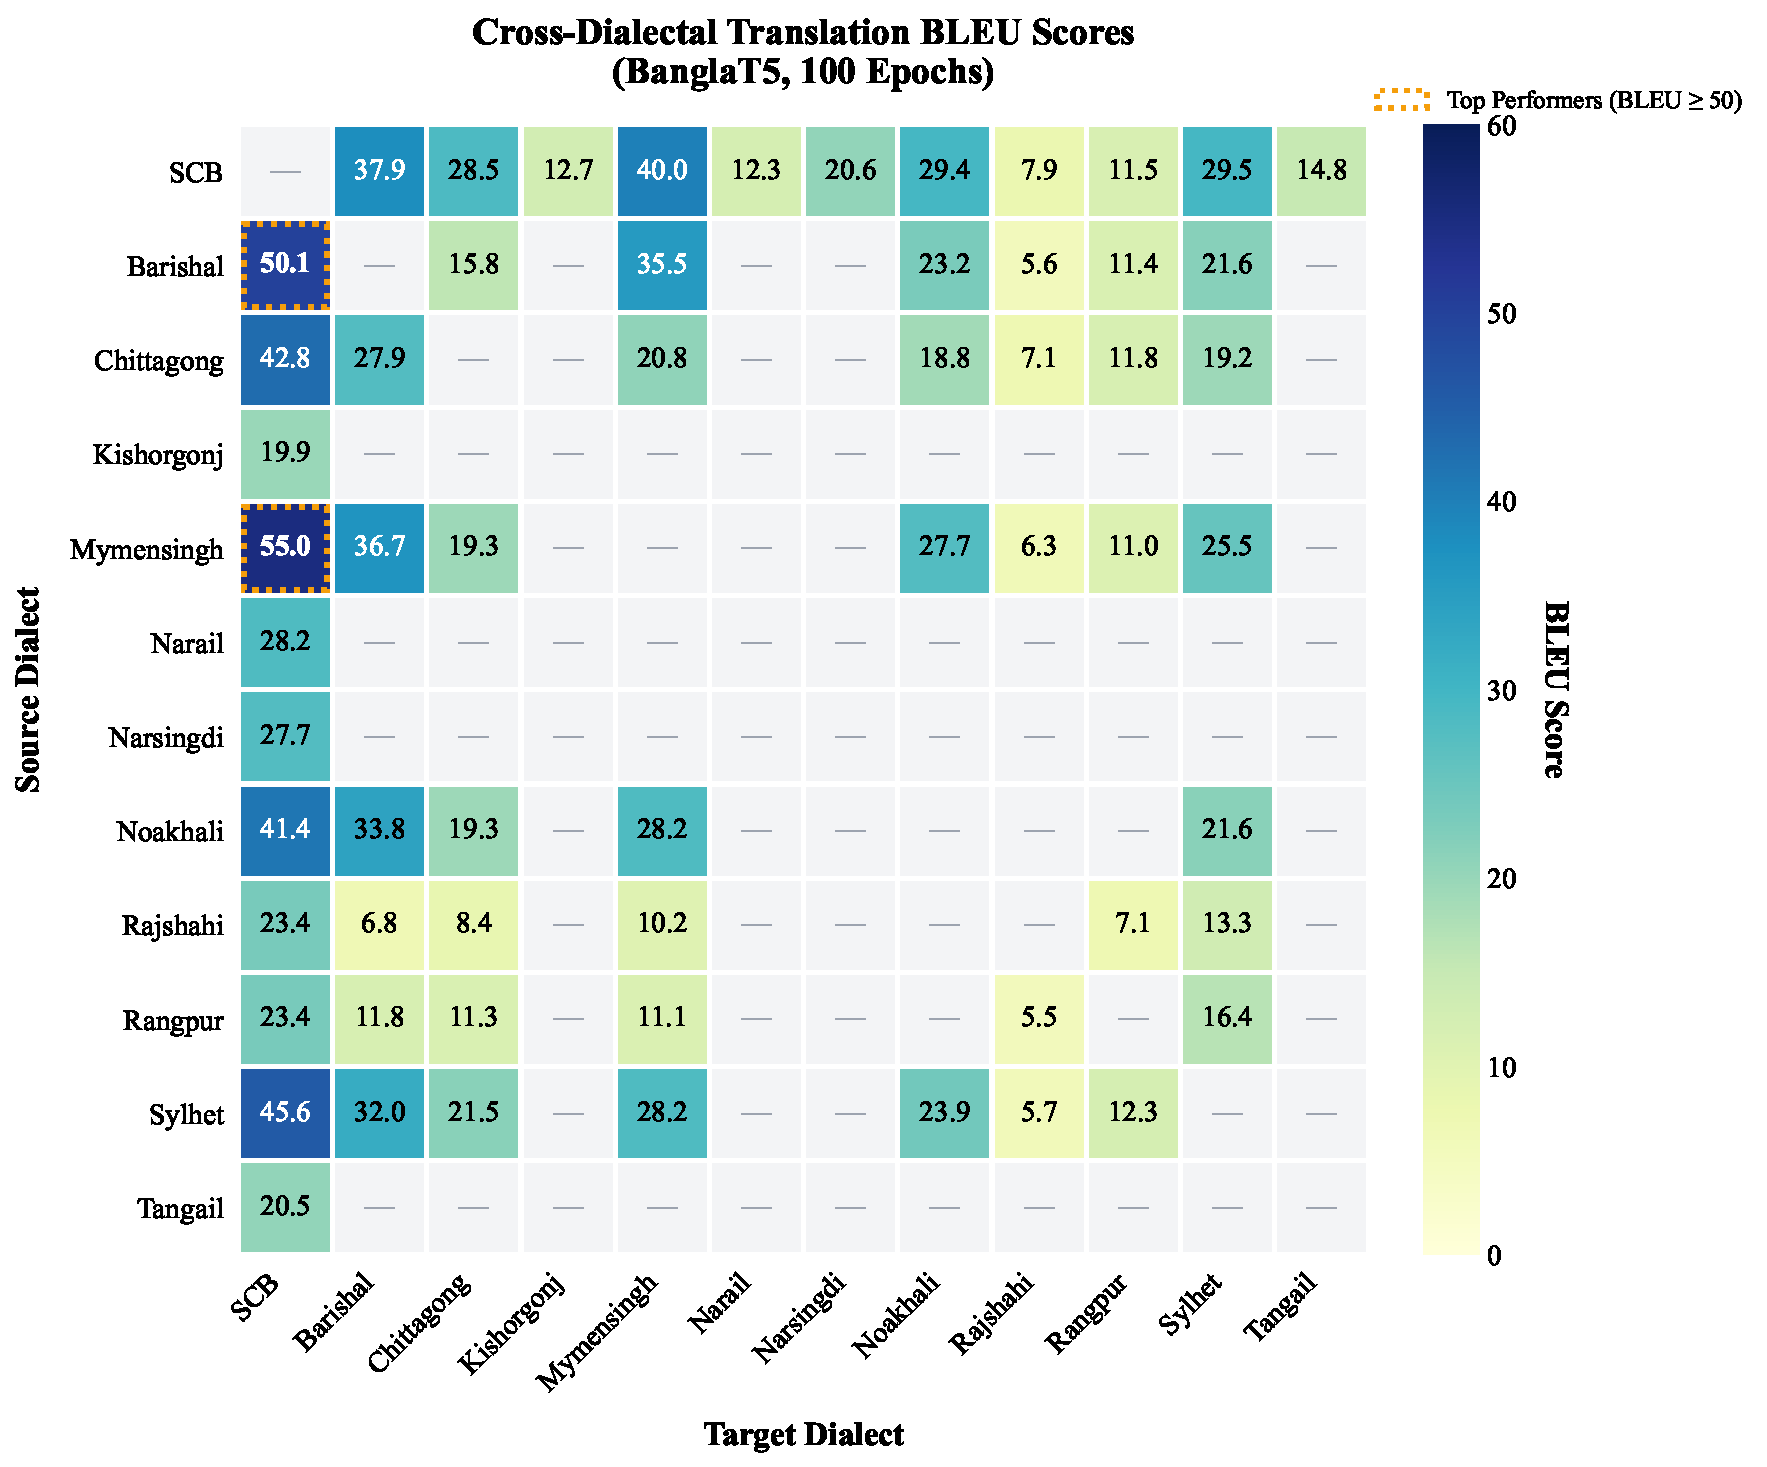
\includegraphics[width=\columnwidth]{graphics/bleu_heatmap.pdf}
  \caption{Cross-dialectal BLEU heatmap (BanglaT5, 100 epochs). Darker shading indicates higher quality; proximate dialects achieve the highest scores.}
  \label{fig:bleu_heatmap}
\end{figure}

\subsection{Error Analysis}
Manual analysis of 200 high-TER failure cases identified five error categories (Fig.~\ref{fig:error_analysis}): \textit{morphological inflection errors} (38\%)---correct roots with wrong dialectal suffixes; \textit{lexical mismatch} (26\%)---region-inappropriate SCB synonyms; \textit{syntactic reordering} (18\%)---incorrect constituent order; \textit{partial translation} (12\%)---mixed source/target segments in low-resource pairs; and \textit{hallucination} (6\%)---semantically unrelated tokens with short or idiomatic inputs~\cite{koehn-knowles-2017-six}.

\begin{figure}[t]
  \centering
  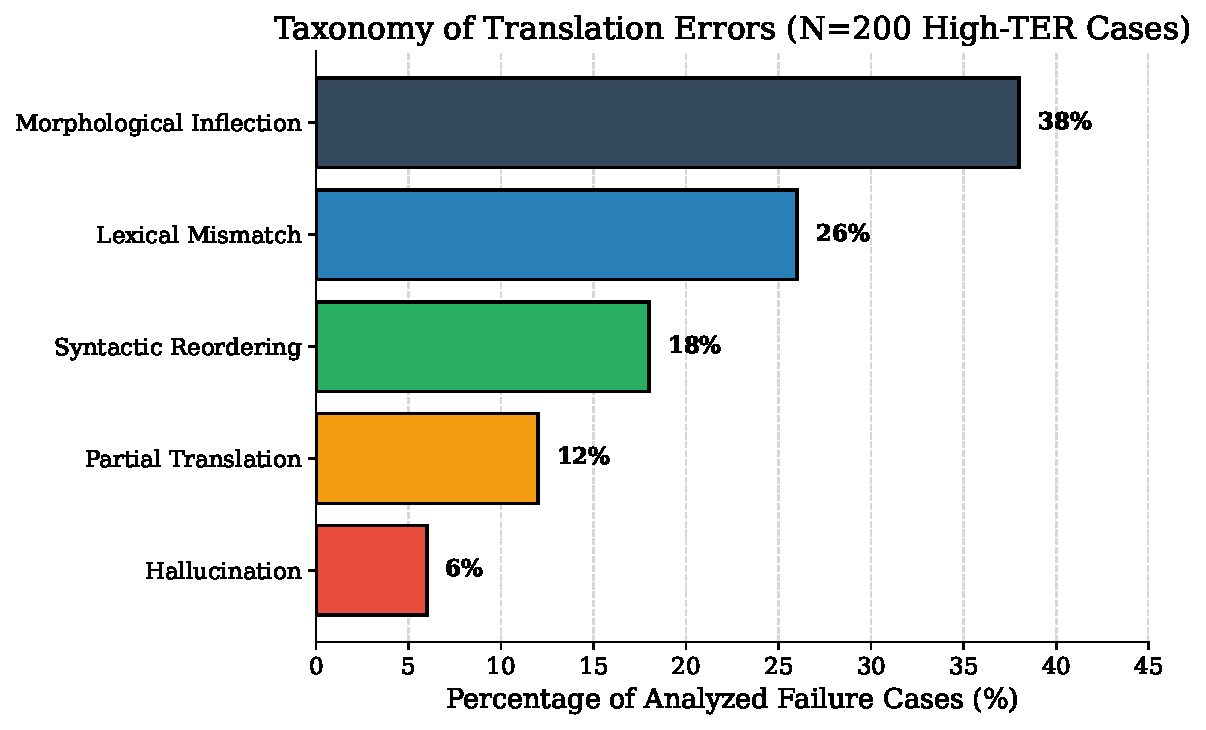
\includegraphics[width=0.85\columnwidth]{graphics/error_taxonomy.pdf}
  \caption{Distribution of translation errors across five linguistic failure categories from 200 high-TER failure cases.}
  \label{fig:error_analysis}
\end{figure}

\subsection{Dataset Scaling Analysis}
A controlled scaling experiment (500--4,499 sentence pairs, four dialects plus SCB) under two DoRA configurations ($r{=}8, \alpha{=}16$ and $r{=}64, \alpha{=}128$) reveals that BLEU improves by up to 140\% (11.47$\rightarrow$27.55) as data scales from 500 to 4,499 pairs (Fig.~\ref{fig:scaling}). The steepest gains occur between 500--2,000 samples, with diminishing returns beyond 3,000, suggesting a practical saturation threshold. The higher-capacity $r{=}64$ configuration consistently outperforms $r{=}8$ by 1--2 BLEU points.

\begin{figure}[t]
  \centering
  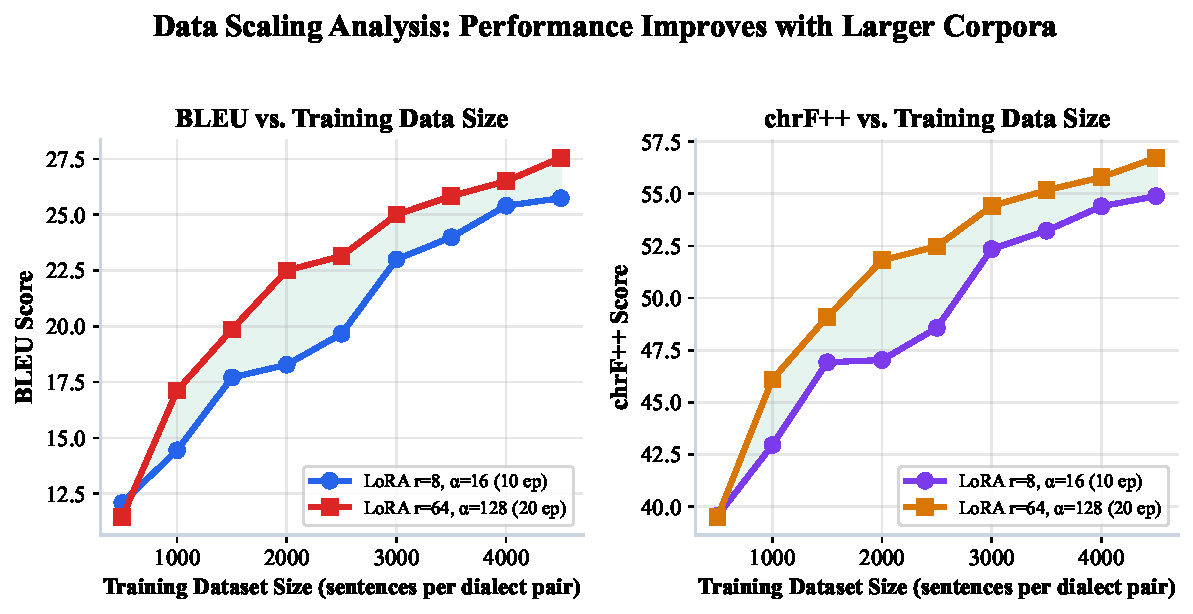
\includegraphics[width=\columnwidth]{graphics/dataset_scaling.pdf}
  \caption{BLEU and chrF++ as a function of training data volume for two DoRA configurations, showing diminishing returns beyond $\sim$3,000 samples.}
  \label{fig:scaling}
\end{figure}

\subsection{Comparison with Prior Work}
Table~\ref{tab:sota} benchmarks our results against recent state-of-the-art systems. The proposed system achieves 29.26 BLEU and 57.26 chrF++, surpassing the best prior result (23.67 BLEU, BanglaCHQ-Prantik~\cite{mahjabin2025banglachq}) by 5.59 BLEU points (23.6\% relative improvement) while covering 12 dialects versus 2--5 in prior work.

\begin{table}[t]
\centering
\caption{Comparison with state-of-the-art benchmarks. Direct comparison should be interpreted cautiously as different works use different test sets.}
\label{tab:sota}
\small
\begin{tabular}{lccc}
\toprule
\textbf{System} & \textbf{Dialects} & \textbf{BLEU} & \textbf{chrF++} \\
\midrule
Vashantor~\cite{faria2025vashantor}     & 5  & 15.42 & 40.15 \\
BhasaBodh~\cite{bhuiyan2025bhasabodh}   & 2  & 17.80 & 43.50 \\
BanglaCHQ~\cite{mahjabin2025banglachq}  & 2  & 23.67 & 48.90 \\
\rowcolor{gray!15} \textbf{Ours}        & \textbf{12} & \textbf{29.26} & \textbf{57.26} \\
\bottomrule
\end{tabular}
\end{table}

\section{Deployment}

The final system was deployed as an interactive web application\footnote{\url{https://bangla-regional-translator.streamlit.app/}} providing real-time translation across 12 dialects. Source code is available at GitHub\footnote{\url{https://github.com/secrakib/Defence_Translator_App}}. The fine-tuned BanglaT5 model with merged DoRA weights was converted to the CTranslate2~\cite{klein-etal-2017-opennmt} inference engine and quantized from FP32 to INT8 precision~\cite{Jacob_2018_CVPR}, reducing peak RAM by over 65\% (operating under 1.5~GB) while accelerating CPU inference by $\sim$3.2$\times$ without perceptible quality degradation. For long documents, a dynamic sentence segmentation pipeline splits input at Bangla boundary delimiters, independently translates each chunk via beam search ($B{=}4$, length penalty $\alpha{=}0.8$, repetition penalty $\beta{=}1.2$), and concatenates the results. Empirical benchmarks show latency of $\sim$900~ms for short sentences (10 words) scaling to $\sim$3,200~ms for long paragraphs (60 words) on standard cloud CPU instances.

\section{Limitations and Future Work}

Several limitations merit acknowledgment. The dataset retains a 21:1 imbalance ratio between SCB and the least represented dialects (500 entries each for Narail, Tangail), constraining generalization. BanglaT5's 32K vocabulary, though superior to multilingual alternatives, was trained on Standard Bangla and may suboptimally segment highly divergent dialectal morphemes. The system operates exclusively on orthographic text, disregarding phonological richness. No formal human evaluation was conducted~\cite{mathur-etal-2020-tangled}.

Future work includes community-driven annotation campaigns; data augmentation via back-translation~\cite{sennrich-etal-2016-improving} and LLM-generated synthetic data~\cite{brown2020language}; multimodal integration with ASR/TTS~\cite{radford2023robust}; formal human evaluation using MQM frameworks~\cite{burchardt-2013-multidimensional}; and cross-lingual transfer from typologically related Indo-Aryan languages.

\section{Conclusion}

This paper presented a comprehensive framework for poly-dialectal neural machine translation in Bangla. We constructed the largest multi-dialect parallel corpus (51,531 pairs, 12 dialects), integrating seven datasets and introducing 2,500 expert-verified pairs for five previously unaddressed dialects. Systematic benchmarking demonstrated that the 247M-parameter BanglaT5 outperforms NLLB-200 (615M) by 51.8\% and mBART-50 (611M) by 145.7\% in BLEU, confirming that language-specific pre-training provides a stronger foundation for intra-language dialectal translation. Extended 100-epoch DoRA fine-tuning achieved state-of-the-art scores of 29.26 BLEU and 57.26 chrF++, surpassing the best prior result by 5.59 BLEU points. Cross-dialectal analysis revealed morphological proximity as the primary determinant of translation quality, and a controlled scaling study established diminishing returns near the 3,000-sample threshold. The system was deployed as a publicly accessible, INT8-quantized web application supporting real-time, multi-directional translation across 12 dialects---including direct dialect-to-dialect paths---constituting a concrete step toward digital inclusion for marginalized Bangla dialect communities.

\section*{Data Availability}
The multi-dialect parallel corpus is publicly available at \url{https://data.mendeley.com/datasets/v9cf66fk2t/2}.

\bibliographystyle{IEEEtran}
\bibliography{biblography}

\end{document}
